\documentclass[12pt,a4paper,openany,oneside]{book}

%------------------------------------------------------------------------------%
%                                                                              %
%   LaTeX Template for Bachlor Thesis of Northwestern Polytechnical University %
%   Using XeLeTeX + MakeIndex + BibTeX, or Using CTeX v2.9.2.164               %
%   Version: 1.3.0                                                             %
%                                                                              %
%------------------------------------------------------------------------------%
%   Copyright 2016 by Shangkun Shen, MIT-LICENSE(see mit-license.polossk.com)  %
%------------------------------------------------------------------------------%


%---------------------------------纸张大小设置---------------------------------%
\usepackage{geometry}
    % 普通A4格式缩进
    % \geometry{left=2.5cm,right=2.5cm,top=2.5cm,bottom=2.5cm}
    % 论文标准缩进
    \geometry{left=1.25in,right=1.25in,top=1in,bottom=1.5in}
%------------------------------------------------------------------------------%


%----------------------------------必要库支持----------------------------------%
\usepackage{amsmath}
\usepackage{amssymb}
\usepackage{amsfonts}
\usepackage{mathrsfs}
\usepackage{bm}
\usepackage{xcolor}
\usepackage{tikz}
\usepackage{layouts}
\usepackage[numbers,sort&compress]{natbib}
\usepackage{clrscode}
\usepackage{gensymb}
%------------------------------------------------------------------------------%


%--------------------------------设置标题与目录--------------------------------%
\usepackage[sf]{titlesec}
\usepackage{titletoc}
%------------------------------------------------------------------------------%


%--------------------------------添加书签超链接--------------------------------%
\usepackage[unicode=true,colorlinks=false,pdfborder={0 0 0}]{hyperref}
    % 在此处修改打开文件操作
    \hypersetup{
        bookmarks=true,         % show bookmarks bar?
        pdftoolbar=true,        % show Acrobat’s toolbar?
        pdfmenubar=true,        % show Acrobat’s menu?
        pdffitwindow=true,      % window fit to page when opened
        pdfstartview={FitH},    % fits the width of the page to the window
        pdfnewwindow=true,      % links in new PDF window
    }
    % 在此处添加文章基础信息
    \hypersetup{
        pdftitle={title},
        pdfauthor={author},
        pdfsubject={subject},
        pdfcreator={creator},
        pdfproducer={producer},
        pdfkeywords={key1  key2  key3}
    }
%------------------------------------------------------------------------------%


%---------------------------------设置字体大小---------------------------------%
\usepackage{type1cm}
% 字号与行距,统一前缀s(a.k.a size)
\newcommand{\sChuhao}{\fontsize{42pt}{63pt}\selectfont}         % 初号, 1.5倍
\newcommand{\sYihao}{\fontsize{26pt}{36pt}\selectfont}          % 一号, 1.4倍
\newcommand{\sErhao}{\fontsize{22pt}{28pt}\selectfont}          % 二号, 1.25倍
\newcommand{\sXiaoer}{\fontsize{18pt}{18pt}\selectfont}         % 小二, 单倍
\newcommand{\sSanhao}{\fontsize{16pt}{24pt}\selectfont}         % 三号, 1.5倍
\newcommand{\sXiaosan}{\fontsize{15pt}{22pt}\selectfont}        % 小三, 1.5倍
\newcommand{\sSihao}{\fontsize{14pt}{21pt}\selectfont}          % 四号, 1.5倍
\newcommand{\sHalfXiaosi}{\fontsize{13pt}{16.25pt}\selectfont}  % 半小四, 1倍
\newcommand{\sXiaosi}{\fontsize{12pt}{14.4pt}\selectfont}       % 小四, 1.25倍
\newcommand{\sLargeWuhao}{\fontsize{11pt}{11pt}\selectfont}     % 大五, 单倍
\newcommand{\sWuhao}{\fontsize{10.5pt}{10.5pt}\selectfont}      % 五号, 单倍
\newcommand{\sXiaowu}{\fontsize{9pt}{9pt}\selectfont}           % 小五, 单倍
%------------------------------------------------------------------------------%


%---------------------------------设置中文字体---------------------------------%
\usepackage{fontspec}
\usepackage[SlantFont,BoldFont,CJKchecksingle,CJKnumber]{xeCJK}
% 使用 Adobe 字体
\newcommand\adobeSog{Adobe Song Std}
\newcommand\adobeHei{Adobe Heiti Std}
\newcommand\adobeKai{Adobe Kaiti Std}
\newcommand\adobeFag{Adobe Fangsong Std}
\newcommand\codeFont{Consolas}
% 设置字体
\defaultfontfeatures{Mapping=tex-text}
\setCJKmainfont[ItalicFont=\adobeKai, BoldFont=\adobeHei]{\adobeSog}
\setCJKsansfont[ItalicFont=\adobeKai, BoldFont=\adobeHei]{\adobeSog}
\setCJKmonofont{\codeFont}
\setmonofont{\codeFont}
% 设置字体族
\setCJKfamilyfont{song}{\adobeSog}      % 宋体  
\setCJKfamilyfont{hei}{\adobeHei}       % 黑体  
\setCJKfamilyfont{kai}{\adobeKai}       % 楷体  
\setCJKfamilyfont{fang}{\adobeFag}      % 仿宋体
% 用于页眉学校名,特殊字体,powerby https://github.com/ecomfe/fonteditor
\setCJKfamilyfont{nwpu}{nwpuname}
% 新建字体命令,统一前缀f(a.k.a font)
\newcommand{\fSong}{\CJKfamily{song}}
\newcommand{\fHei}{\CJKfamily{hei}}
\newcommand{\fFang}{\CJKfamily{fang}}
\newcommand{\fKai}{\CJKfamily{kai}}
\newcommand{\fNWPU}{\CJKfamily{nwpu}}
%------------------------------------------------------------------------------%


%------------------------------添加插图与表格控制------------------------------%
\usepackage{graphicx}
\usepackage[font=small,labelsep=quad]{caption}
\usepackage{wrapfig}
\usepackage{multirow,makecell}
\usepackage{longtable}
\usepackage{booktabs}
\usepackage{tabularx}
\usepackage{setspace}
%------------------------------------------------------------------------------%


%---------------------------------添加列表控制---------------------------------%
\usepackage{enumerate}
\usepackage{enumitem}
%------------------------------------------------------------------------------%


%---------------------------------设置引用格式---------------------------------%
\renewcommand\figureautorefname{图}
\renewcommand\tableautorefname{表}
\renewcommand\equationautorefname{式}
\newcommand\myreference[1]{[\ref{#1}]}
\newcommand\eqrefe[1]{式(\ref{#1})}
\renewcommand\theequation{\thechapter-\arabic{equation}}
% 增加 \ucite 命令使显示的引用为上标形式
\newcommand{\ucite}[1]{$^{\mbox{\scriptsize \cite{#1}}}$}
%------------------------------------------------------------------------------%


%--------------------------------设置定理类环境--------------------------------%
\usepackage[amsmath,thmmarks]{ntheorem}
\newtheorem{myexample}{例}
\newtheorem{thm}{定理}
%------------------------------------------------------------------------------%


%--------------------------设置中文段落缩进与正文版式--------------------------%
\XeTeXlinebreaklocale "zh"       %使用中文的换行风格
\XeTeXlinebreakskip = 0pt plus 1pt    %调整换行逻辑的弹性大小
% \xeCJKcaption{gb_452}
\usepackage{indentfirst}
\setlength{\parindent}{26pt}
\setlength{\parskip}{3pt plus 1pt minus 1pt} % 段落间距
\renewcommand{\baselinestretch}{1.25} % 行距
%------------------------------------------------------------------------------%


%----------------------------设置段落标题与目录格式----------------------------%
\setcounter{secnumdepth}{3}
\setcounter{tocdepth}{2}


% 正文中标题格式,毋需标号
% \titleformat{\section}[hang]{\fHei \sf \sSihao}
%     {\sSihao }{0.5em}{}{}
% \titleformat{\subsection}[hang]{\fHei \sf \sHalfXiaosi}
%     {\sHalfXiaosi }{0.5em}{}{}
% \titleformat{\subsubsection}[hang]{\fHei \sf}
%     {\thesubsubsection }{0.5em}{}{}
% 正文中标题格式,需要标号

\newcommand\chapterID[1]{第\CJKnumber{#1}章}
\renewcommand{\chaptername}{第\CJKnumber{\thechapter}章}
\renewcommand{\figurename}{图}
\renewcommand{\tablename}{表}
\renewcommand{\bibname}{参考文献}
\renewcommand{\contentsname}{目~录}
\newcommand{\keywords}[1]{\\ \\ \textbf{关~键~词}:#1}


\titleformat{\chapter}[hang]{\normalfont\sSanhao\filcenter\fHei\bf}%
    {\sSanhao{\chaptertitlename}}{20pt}{\sSanhao}
\titleformat{\section}[hang]{\fHei \bf \sSihao}%
    {\sSihao \thesection}{0.5em}{}{}
\titleformat{\subsection}[hang]{\fHei \bf \sHalfXiaosi}%
    {\sHalfXiaosi \thesubsection}{0.5em}{}{}
\titleformat{\subsubsection}[hang]{\fHei \bf}%
    {\thesubsubsection }{0.5em}{}{}


% 缩小正文中各级标题之间的缩进
\titlespacing{\chapter}{0pt}{-3ex plus .1ex minus .2ex}{0.25em}
\titlespacing{\section}{0pt}{-0.2em}{0em}
\titlespacing{\subsection}{0pt}{0.5em}{0em}
\titlespacing{\subsubsection}{0pt}{0.25em}{0pt}

% 定义目录中各级标题之间的格式以及缩进
% \dottedcontents{chapter}[0.0em]{\fHei\vspace{0.5em}}{0.0em}{5pt}
\dottedcontents{section}[1.16cm]{}{1.8em}{5pt}
\dottedcontents{subsection}[2.00cm]{}{2.7em}{5pt}
\dottedcontents{subsubsection}[2.86cm]{}{3.4em}{5pt}
\titlecontents{chapter}[0pt]{\fHei\vspace{0.5em}}%
    {\contentsmargin{0pt}\fHei\makebox[0pt][l]{\chapterID{\thecontentslabel}}\hspace{3.8em}}%
    {\contentsmargin{0pt}\fHei}%
    {\titlerule*[.5pc]{.}\contentspage}[\vspace{0em}]


%------------------------------------------------------------------------------%

%---------------------------------设置页眉页脚---------------------------------%
\usepackage{fancyhdr}
\usepackage{fancyref}
%\addtolength{\headsep}{-0.1cm}          %页眉位置
%\addtolength{\footskip}{-0.1cm}         %页脚位置
\addtolength{\topmargin}{0.5cm}
\newcommand{\makeheadrule}{
    \makebox[0pt][l]{\rule[.7\baselineskip]{\headwidth}{0.8pt}}
    \vskip-.8\baselineskip
}
\makeatletter
\renewcommand{\headrule}{%
    {
        \if@fancyplain\let\headrulewidth\plainheadrulewidth\fi
        \makeheadrule
    }
}
\pagestyle{fancyplain}
\fancyhf{}
\fancyfoot[C,C]{\sWuhao-~\thepage~-}
% 后续文字可以自行修改
\chead{\sSanhao\raisebox{0.04cm}{\fNWPU 西北工业大学} \fSong {\bf 本科毕业设计论文}}
%------------------------------------------------------------------------------%


%-------------------------------数学符号格式控制-------------------------------%
\usepackage{bm}
\def\mathbi#1{\textbf{\em #1}}
% Caligraphic letters:      \mathcal{A}
% Mathbb letters:           \mathbb{A}
% Mathfrak letters:         \mathfrak{A}
% Math Sans serif letters:  \mathsf{A}
% MAth bold letters:        \mathbf{A}
% Math bold italic letters: \mathbi{A}
%------------------------------------------------------------------------------%


%-------------------------------数学特殊符号控制-------------------------------%
\newcommand\mi{{\mathrm i}}             % constant i
\newcommand\me{{\mathrm e}}             % constant e
\newcommand\mreal{{\mathbb R}}          % constant real set R
\newcommand\mhilb{{\mathbb H}}          % constant hilbert set H
\newcommand\mcond{{\mathrm{Cond.}}}     % condition symbol
\newcommand\mconst{{\mathrm{const}}}    % constant symbol
\newcommand\mve{{\bm e}}                % vector e
\newcommand\mvu{{\bm u}}                % vector u
\newcommand\mvv{{\bm v}}                % vector v
\newcommand\mvw{{\bm w}}                % vector w
\newcommand\mvx{{\bm x}}                % vector x
\newcommand\mvy{{\bm y}}                % vector y
\newcommand\mvz{{\bm z}}                % vector z
\newcommand\mvzero{{\bm 0}}             % vector 0
\newcommand\mvone{{\bm 1}}              % vector 1
\newcommand\mvalpha{{\bm \alpha}}       % vector alpha
\newcommand\mvomega{{\bm \omega}}       % vector omega
\newcommand\mma{{\mathbf A}}            % matrix A
\newcommand\mmb{{\mathbf B}}            % matrix B
\newcommand\mmd{{\mathbf D}}            % matrix D
\newcommand\mmh{{\mathbf H}}            % matrix H
\newcommand\mmi{{\mathbf I}}            % matrix I
\newcommand\mmk{{\mathbf K}}            % matrix K
\newcommand\mml{{\mathbf L}}            % matrix L
\newcommand\mmo{{\mathbf O}}            % matrix O
\newcommand\mmp{{\mathbf P}}            % matrix P
\newcommand\mms{{\mathbf S}}            % matrix S
\newcommand\mmt{{\mathbf T}}            % matrix T
\newcommand\mmtt{{{\mathbf T}^T}}       % matrix T^T
\newcommand\mmu{{\mathbf U}}            % matrix U
\newcommand\mmv{{\mathbf V}}            % matrix V
\newcommand\mmw{{\mathbf W}}            % matrix W
\newcommand\mmx{{\mathbf X}}            % matrix X
\newcommand\mmy{{\mathbf Y}}            % matrix Y
\newcommand\mmz{{\mathbf Z}}            % matrix Z
\newcommand\mmlambda{{\bm \Lambda}}     % matrix \Lambda
\newcommand\mf{{\mathcal{F}}}           % mathcal F
\newcommand\mr{{\mathcal{R}}}           % mathcal R
\DeclareMathOperator\diff{d\!}          % operator diff
\DeclareMathOperator\Diff{D\!}          % operator Diff
\DeclareMathOperator\Expect{E}          % operator Expect
\DeclareMathOperator\diag{diag}         % operator diag
\DeclareMathOperator\eig{eig}           % operator eig
\DeclareMathOperator\lcm{lcm}           % operator lcm
\DeclareMathOperator\tr{tr}             % operator tr
\DeclareMathOperator\var{var}           % operator var
\DeclareMathOperator\cov{cov}           % operator cov
\DeclareMathOperator\mean{mean}         % operator mean
\DeclareMathOperator*{\argmin}{argmin}  % operator argmin
\DeclareMathOperator{\dist}{dist}       % operator dist
\allowdisplaybreaks[4]
%------------------------------------------------------------------------------%

%----------------------------------其他补充设置--------------------------------%
% 重置列表环境的间隔
% \let\orig@Itemize =\itemize
% \let\orig@Enumerate =\enumerate
% \let\orig@Description =\description

% \def\Myspacing{
%     \itemsep=1.5ex \topsep=-0.5ex \partopsep=0pt \parskip=0pt \parsep=0.5ex
% }

% \def\newitemsep{
%     \renewenvironment{itemize}{\orig@Itemize\Myspacing}{\endlist}
%     \renewenvironment{enumerate}{\orig@Enumerate\Myspacing}{\endlist}
%     \renewenvironment{description}{\orig@Description\Myspacing}{\endlist}
% }

% \def\olditemsep{
%     \renewenvironment{itemize}{\orig@Itemize}{\endlist}
%     \renewenvironment{enumerate}{\orig@Enumerate}{\endlist}
%     \renewenvironment{description}{\orig@Description}{\endlist}
% }

% \newitemsep
% 下划线
\newcommand\dlmu@underline[2][5cm]{\hskip1pt\underline{\hb@xt@ #1{\hss#2\hss}}\hskip3pt}
\let\coverunderline\dlmu@underline
%------------------------------------------------------------------------------%



%----------------------------------添加代码控制--------------------------------%
\usepackage{listings}
\lstset{
    basicstyle=\footnotesize\ttfamily,
    %numbers=left,
    %numberstyle=\tiny,
    %numbersep=5pt,
    tabsize=4,
    extendedchars=true,
    breaklines=true,
    keywordstyle=\color{blue},
    numberstyle=\color{purple},
    commentstyle=\color{olive},
    stringstyle=\color{orange}\ttfamily,
    showspaces=false,
    showtabs=false,
    framexrightmargin=5pt,
    framexbottommargin=4pt,
    showstringspaces=false
    escapeinside=`', %逃逸字符(1左面的键),用于显示中文
}
\renewcommand{\lstlistingname}{CODE}
\lstloadlanguages{% Check Dokumentation for further languages, page 12
    Pascal, C++, Java, Ruby, Python, Matlab, R
}
%------------------------------------------------------------------------------%

\renewcommand\arraystretch{1.4}
\renewcommand{\thefigure}{\thechapter-\arabic{figure}}
\renewcommand{\thetable}{\thechapter-\arabic{table}}
\captionsetup[table]{labelfont=bf,textfont=bf}
\graphicspath{{figures/}}

\endinput
% 这是简单的 thesis(article) 的导言区设置,不能单独编译。


% 仅用于测试
\usepackage{blindtext}

\title{\textsf{比如我举个例子}}
\author{{\kai 谁知道呢}}
\date{May 20, 20xx}

\begin{document}

\sloppy

\pagenumbering{Roman}

% 封皮
\frontmatter
% 本科毕业设计论文模板
% 封皮
\begin{titlepage}
	\voffset 2.7cm
	\begin{center}
		\begin{center}
			\begin{minipage}[c]{2.64cm}
				\centering
				\resizebox{!}{0.9cm}{ \parbox{0.54cm}{ \begin{tikzpicture}
    \draw[line width=0.10cm] (0, 0) circle (2.0cm);
    % \fill[gray!15] (0, 0) -- (1.3cm,0cm) arc (0:230:1.3cm) -- cycle;
    % \fill[gray!15] (0, 0) -- (1.3cm,0cm) arc (0:-50:1.3cm) -- cycle;
    \foreach \t in {-50, -40, -30, -20, -10, 0, 10, 20, 30, 40, 50, 60, 70, 80, 90, 100, 110, 120, 130, 140, 150, 160, 170, 180, 190, 200, 210, 220, 230}
    {
        \foreach \p/\d in {0/0.01cm, 5/-0.01cm}
        {
            \foreach \r in {1.27cm, 1.17cm, 1.07cm, 0.97cm}
            {
                \fill (\t + \p: \r + \d) circle (0.01cm);
            }
        }
    };
    \draw[line width=0.03cm] (0, 0) circle (1.32cm);
    \fill[white] (0, 0) circle (0.9cm);
    \draw[line width=0.05cm] (0, 0) circle (0.9cm);
    \fill[black] (-0.50, -0.73) .. controls (-0.35, -0.81) ..
        (-0.2, -0.80) .. controls (0.15, -0.70) and (0.20, -0.60) .. 
        (0.35, -0.35) .. controls (0.42, -0.24) and (0.60, -0.26) ..
        (0.60, -0.40) .. controls (0.58, -0.50) and (0.49, -0.50) ..
        (0.45, -0.45) .. controls (0.40, -0.68) and (0.75, -0.70) ..
        (0.90, 0.00) arc (360:250:0.9cm);
    \fill (-0.40, -0.40)--(-1.33, -0.40)--(1.00, 1.10)--cycle;
    \fill (-0.37, -0.43)--(-0.20, -0.80)--(1.01, 1.05)--cycle;
    
    \foreach \x/\txt in {0/N, 1/O, 2/R, 3/T, 4/H, 5/W, 6/E, 7/S, 8/T, 9/E, 10/R, 11/N, 12/~, 13/P, 14/O, 15/L, 16/Y, 17/T, 18/E, 19/C, 20/H, 21/N, 22/I, 23/C, 24/A, 25/L, 26/~, 27/U, 28/N, 29/I, 30/V, 31/E, 32/R, 33/S, 34/I, 35/T, 36/Y}
    {
        \node[scale=0.7, rotate=\x*-6.50-245] at (207+\x*-6.50:1.6cm) {\txt};
    };

    \foreach \x/\txt in {0/西, 1/北, 2/工, 3/业, 4/大, 5/学}
    {
        \node[scale=1.25, rotate=\x*18-50] at (225+\x*18:1.65cm) {\fNWPU\txt};
    };

    \foreach \x/\txt in {0/1, 1/9, 2/3, 3/8}
    {
        \node[scale=1, rotate=\x*18-25] at (\x*18-115:1.1cm) {\bfseries\txt};
    };
\end{tikzpicture}

\endinput
% 这是西北工业大学校徽文件,不能单独编译。 } }
				\end{minipage}
				\hskip 0.8cm
				\begin{minipage}[c]{8cm}
				\fontsize{33}{33}\fNWPU 西北工业大学
			\end{minipage}
		\end{center}
		\vskip 0.7cm
		\sChuhao\fSong {\bfseries 本科毕业设计论文}
		\vskip 5cm
		{
		\sSanhao\fHei 题~~目 \hspace{0.2cm}\coverunderline[12.5cm]{题目这种东西随便起一个就行了}
		}
		\vskip 2cm
		{
			\sSihao\fSong 专业名称\coverunderline[5.5cm]{看文档找规律专业}
			\vskip 0.7cm
			\sSihao\fSong 学生姓名\coverunderline[5.5cm]{哦}
			\vskip 0.7cm
			\sSihao\fSong 指导教师\coverunderline[5.5cm]{自学成才}
			\vskip 0.7cm
			\sSihao\fSong 完成时间\coverunderline[5.5cm]{阴吹思婷}
			\vfill
		}
	\end{center}
\end{titlepage}
\fSong \normalsize

\endinput
% 这是封面排版文件,不能单独编译。

\setcounter{page}{1}
\renewcommand{\baselinestretch}{1.25}

% 中文摘要
% 中文摘要
\begin{abstract}
	% 中文 \lipsum[2-3]

	% 摘要——学位论文的简短陈述,应说明该研究工作的目的意义、研究方法、研究成果等,其重点是研究成果,摘要字数一般为硕士论文700~1000字
本文以雷达信号分类识别为主要应用背景,利用深度学习的思想与方法,重点研究了天波超视距雷达地海杂波识别和雷达辐射源识别这两个实际工程问题,具体工作如下:

1)利用天波超视距雷达地海杂波识别结果可以实时准确获得天波雷达的坐标配准修正系数,进而有效提高目标定位精度。
本文在对地海杂波频谱实际数据深入分析的基础上,对原始频谱数据首先进行清洗、裁剪、融合等预处理步骤,然后构建了一个具有六层的深度卷积神经网络分类器并利用具有自适应学习率的算法进行学习,同时结合地海杂波这一实际工程问题对分类阈值进行调整,最后对输出结果以分类精度和与实际地图的匹配精度两个层面进行衡量。
实验结果表明,基于深度卷积神经网络的地海杂波识别算法在电离层环境较差的情况下仍具有较高的识别精度。

2)为了克服大量数据进行标记的成本过高以及部分数据难以人工准确标注的问题,本文进一步提出了基于深度嵌入卷积的地海杂波聚类方法。
通过在地海杂波数据中包含空间、时间信息,添加卷积层、卷积转置层和全连接层,设计了一个以端到端方式训练的卷积自编码器来从未标记的数据中学习特征,并将KL散度与重构损失两部分结合设计了一个新的损失函数。
利用天波超视距雷达的实际地海杂波数据的实验结果表明了深度嵌入卷积聚类算法的有效性。

3)针对复杂电磁环境下辐射源的识别面临的电磁信号干扰大、雷达信号参数相近以及工程中存在未知类别的辐射源等问题与挑战,本文提出了基于深度学习的辐射源个体识别算法。
通过对现有辐射源信号进行分析,利用其模糊函数切片这一脉内细微特征作为训练样本,构建了一个具有10层的一维卷积神经网络作为主分类器来对输入信号做初次分类,其后跟随一个支持向量机分类器作为Meta-Recognition,实现对辐射源中未知类别的辨别。
通过多架飞机的气象雷达辐射源的实际数据证明了本文算法分类的准确性。



	\begin{keywords}
		雷达信号分类, 天波雷达地海杂波识别, 雷达辐射源分类, 深度学习, 卷积神经网络
	\end{keywords}
\end{abstract}
% 英文摘要
% !Mode:: "TeX:UTF-8"

% 英文摘要
\begin{Abstract}
Under the background of radar signal classification, this paper focuses on sea/land clutter recognition for Over-the-Horizon Radar(OTHR) and specific emitter identification using deep learning methodology, as follows:


1)The results of OTHR sea/land clutter recognition can be used for coordinate registration, which can help improve the target positioning accuracy effectively.
Based on the analysis of sea/land clutter spectrum data, a six-layer deep convolution neural network classifier is constructed. The original spectrum data is preprocessed by cleansing, trimming, and fusion.
Adaptive Moment Estimation method is used to train the network, which can give a stable learning rate.
As a real-world project, the classification threshold is adjusted according to the features of clutter. The results are evaluated by the classification accuracy and the matching accuracy with actual map.
Experimental results show that the clutter recognition algorithm based on deep convolution neural network still has high recognition accuracy under poor ionospheric environment.

2)In order to overcome the high cost of labeling large amounts of data and the difficult to label some data  accurately manually, this paper further proposed a deep embeddeding convolution method for sea/land clutter clustering.
Spatial locations and time sequences information is added to original clutter spectrum data. The network contains convolutional layer, deconvolutional layer and fully connected layer.
A convolutional autoencoders structure is developed to learn embedded features in an end-to-end way.
The experimental results show the effectiveness of deep embeddeding convolution clustering method.

3)In order to solve the problems of recognizing emitters in similar radar signal parameters and the existence of unknown types emitterin complex electromagnetic environment, this paper proposed a specific emitter identification method based on deep learning.
By analyzing the signal of the specific emitters and using the ambiguity function slice as feature vectors,
a 10-layer one-dimensional convolution neural network is constructed as the primary classifier to classify the input signals firstly. Unknown types of specific emitters are identified by a support vector machine classifier as Meta-Recognition.
The classification accuracy of the algorithm proposed in this paper is high in the experiments of meteorological radars from multiple aircraft.



	\begin{Keywords}
		Radar Signal Classification, Sea/Land Clutter Recognition for Over-The-Horizon Radar, Specific Emitter Identification, Deep Learning, Convolutional Neural Networks
	\end{Keywords}
\end{Abstract}

\renewcommand{\baselinestretch}{1.25}
\fontsize{12pt}{12pt}\selectfont
\phantomsection
\addcontentsline{toc}{chapter}{\fHei 目录}
\tableofcontents
\clearpage
\mainmatter

\renewcommand{\baselinestretch}{1.0}

\sHalfXiaosi\fSong

% 正文内容
\chapter{绪论}
\section{引言}
而是
\section{天波超视距雷达地海杂波识别}

超视距雷达(OTHR)在高频段运行,能够通过电离层反射检测和定位超过地平线的地区的移动目标,因此在持续监测中起着重要作用\cite{headrick1974over, fabrizio2013high}。 然而,电磁信号通过电离层的传播导致强制性程序,用于目标定位的坐标登记〜(CR),因为地面坐标系中的目标位置(即纬度和经度)是必需的,但是OTHR接收测量 倾斜坐标系〜(即倾斜方位角和倾斜范围)\cite{krolik1997maximum}。 要执行CR,必须调用两个子步骤,(1)为每个测量或目标状态估计选择正确的电离层传播模式,(2)将测量或目标的状态估计从倾斜坐标系转换为地面坐标系。

% In general, a sub-system consists of several ionosondes is deployed and operated with OTHR to provide the information required by CR. The information includes the possible ionosphere propagation modes and the corresponding parameters for each propagation mode, such as the height of each layer of the ionosphere \cite{wheadon1994ionospheric}. OTHR takes such information from ionosondes as the input of it and achieves CR. There are two factors that may deteriorate the localization performance of OTHR using ionosondes. The first one is that the deployment of ionosondes is restricted to available areas. For example, ionosondes can not be deployed in the sea or hostile areas. The ionosphere's parameters of unavailable areas are often obtained by interpolation with those of available areas based on statistical ionospheric models, making the information input into CR inaccurate. The second one is that the independent operation of ionosondes from OTHR results in consistency on the number of propagation modes and inaccuracy on the parameters for each propagation mode. More specifically, the propagation modes recognized by ionosondes may not the same as the propagation modes that the measurements received by the OTHR originate from. Therefore, to reduce the chances of incorrect identification of propagation mode for each measurement or state estimate, and the effect caused by the error of parameters provided by ionosondes so that improve the accuracy of CR, alternative methodologies have to be sought.
一般来说,由OTHR部署和操作的几个离子键合子的子系统提供CR所需的信息。该信息包括可能的电离层传播模式和每个传播模式的相应参数,例如电离层的每层的高度\cite{wheadon1994ionospheric}。 OTHR从Ionosondes获取这些信息作为其输入,并实现CR。有两个因素可能会降低使用离子键的OTHR的定位性能。第一个是离子质子的部署仅限于可用的区域。例如,离子潜能不能部署在海洋或敌对区域。不可用区域的电离层参数常常通过基于统计电离层模型的可用区域插值得到,使信息输入到CR不准确。第二个是来自OTHR的离子键的独立操作导致传播模式的数量和每个传播模式的参数的不准确性一致。更具体地说,离子键的识别传播模式可能不同于OTHR所接收的测量的传播模式。因此,为了减少每个测量或状态估计的传播模式的错误识别的机会,以及由离子质子提供的参数的误差引起的影响,从而提高CR的准确性,必须寻求替代方法。

改善CR的一种方法是使用beacons\cite{weijers1995oth}。 OTHR接收信标发送的信号,并在倾斜坐标系中输出其位置上的测量值。 通过将测量与由GPS提供的地面坐标系中的信标的已知位置进行比较,可以实时地进行CR过程的校正。 然而,信标的使用仅限于可用的区域。 此外,需要对信标进行维护。
% One way available to improve CR is using beacons \cite{weijers1995oth}. OTHR receives the signals transmitted by beacons and outputs the measurements on their locations in slant coordinate system. By comparing the measurements with known locations of beacons in ground coordinate system provided by GPS, correction on the CR process can be carry out in real-time. However, the utilization of beacons is restricted to available areas as well. Additionally, maintenance on beacons is needed.

事实上,另一个来源,海洋/陆地的转变,可以被看作是一种被动的信标,因为海洋和陆地的信号是可以识别的,因为同样的原则是适用的。 使用海岸线的CR的想法首先出现在\cite{wheadon1994ionospheric, anderson1995auto},没有详细的结果报告。 巴纳姆等人\cite{barnum1998over}提出了一种基于海/陆杂波识别的CR方法,主要依靠构造杂波模型。 然而,由于电离层状况的复杂性,海/陆杂乱的特征不稳定,例如海杂波,布拉格峰的主要特征之一可能会偏移甚至失去一个峰值。
% In fact, another source, sea/land transitions, can be regarded as a kind of passive beacons since the same principle is applicable if the signals of sea and land are identifiable. The idea of using coastline for CR is first appeared in \cite{wheadon1994ionospheric, anderson1995auto}, where no detailed results were reported. Barnum~{\emph et. al.} \cite{barnum1998over} proposed a CR method based on sea/land clutter identification, which mainly relies on constructing the clutter model. However, due to the complexity of ionospheric situation, the characteristics of the sea/land clutter is not stable, for example, one of the main features of sea clutter, Brag peak, may shift or even lost one peak.

在本文\cite{cuccoli2009over, cuccoli2009over2, cuccoli2010sea, cuccoli2011coordinate}中,我们提出了一种针对Horizon Sky Wave信号实时坐标注册问题的方法。 该方法是基于对雷达覆盖区域内的海陆过渡位移的先验知识,即利用监视区域的地理形态结构,利用其构建二进制掩模,将其用作 接收的雷达回波的地理参考。 概述了基于收到的雷达回波和二进制杂波签名之间的互相关最大化的地理参考算法,以便指出接收到的信噪比和差分海陆反射散射的最小要求 系数。
% In \cite{cuccoli2009over, cuccoli2009over2, cuccoli2010sea, cuccoli2011coordinate}, In this paper, we propose an approach to the problem of real time coordinate registration for Over the Horizon Sky Wave signals. The approach is based on the a priori knowledge of the displacement of the sea-land transitions within the radar coverage area, namely, takes advantage of the geo-morphological structure of the surveillance area, employing it to build a binary mask to be used as a geographic reference for the received radar echo. The georeferencing algorithm, based on the maximization of the cross-correlation between the received radar echo and the binary clutter signatures, is outlined in order to point out the minimum requirements in terms of received signal-to-noise ratio and differential sea-land backscattering coefficient.

在 \cite{cuccoli2009over2}中,我们最近提出了一种基于对海陆过渡位置的先验知识的天空天空雷达(OTHRsw)的接收到的回波的实时协调注册(CR)的相关方法 在雷达覆盖范围内。 在本文中,我们提出了一种软件仿真工具,用于分析不同OTHR情景中提出的CR方法的性能。 软件工具使用简化的电离层模型和表面杂波雷达相互作用的简化模型来模拟单声道OTH雷达传播。 提出并讨论了假设不同表面杂波场景的仿真结果。
% In \cite{cuccoli2009over2}, We recently proposed a correlation method for the real time Coordinate Registration (CR) of the received echo by Over The Horizon Sky Wave Radar (OTHRsw) based on a priori knowledge of the positions of the Sea-Land transitions within the radar coverage area. In this paper we present a software simulation tool developed to analyze the performance of the proposed CR method in different OTHR scenarios. The software tool simulates the monostatic OTH radar propagation using simplified ionospheric models and simplified models of surface clutter radar interactions. Simulation results assuming different surface clutter scenarios are presented and discussed.

在\cite{cuccoli2010sea}中,我们最近提出了一种基于对海上地位的先验知识的Over Horizon Horizon Wave Radar(OTHR-SW)的接收回波的实时协调注册(CR)的相关方法, 雷达覆盖区内的陆地过渡。 在本文中,我们提出了一个模拟器,可以用于现实OTHR场景中提出的CR方法的性能分析。 假设一个单一的海陆转换场景和一个地理上不变的垂直电子密度分布,提出和讨论了一些模拟结果。
% In \cite{cuccoli2010sea}, We recently proposed a correlation method for the real time Coordinate Registration (CR) of the received echo by Over The Horizon Sky Wave Radar (OTHR-SW) based on a priori knowledge of the positions of the sea-land transitions within the radar coverage area. In this paper we present a simulator that can be used for performance analysis of the proposed CR method in realistic OTHR scenarios. Some simulation result are presented and discussed assuming a single sea-land transition scenario and a geographically invariant vertical electron density profile.

% In \cite{cuccoli2011coordinate}, Cuccoli~{\emph et. al.} studied the problem of range coordinate registration leveraging the geomorphological structure of the surveillance area. The geographical information including coastlines is represented by sea/land binary mask, which is further converted to a reference signal depending on the equivalent ionospheric reflection height. The right equivalent ionospheric reflection height is determined by maximizing the cross-correlation between the received radar echo and the surface mask signatures. However, they assume the OTHR transmits single pulse signals and numerical simulation results are provided.
Cuccoli\cite{cuccoli2011coordinate}等人提出利用监控区域的地貌结构研究范围坐标登记问题。 包括海岸线的地理信息由海/陆二进制掩码表示,根据等电离层反射高度进一步转换为参考信号。 通过最大化接收的雷达回波和表面掩模签名之间的互相关来确定正确的等效电离层反射高度。 然而,他们假设OTHR传输单脉冲信号,并提供数值模拟结果。
% In \cite{cacciamano2012coordinate}, Target detection in Over-The-Horizon (OTH) radars is accomplished by tracking returns in slant range, Doppler and azimuth. Coordinate registration (CR) is the process of localizing the target by converting the slant coordinates to ground coordinates for all the frequencies used in transmission. The CR method uses a 3D ray-tracing algorithm which provides the ground range distance reached with a specific transmission frequency and elevation angle. The ray-tracing approach here adopted uses a 3D electron density model variable with height, latitude and longitude. The ray-tracing output is generally affected by errors due to numerical approximations of the 3D ionosphere model and discretization step used to integrate the differential equations of ray-tracing algorithm. Therefore the raw CR diagram suffers from an error which introduces as a consequence a degradation of target localization accuracy. Accordingly, we propose a coordinate registration technique for OTH sky-wave radars based on 3D ray-tracing that uses the sea-land transitions to mitigate the CR errors. The approach is based on the a priori knowledge of actual group delays relative to the sea-land transition within the area illuminated by the radar antenna beam. The method takes advantage of the geomorphological structure of the surveillance area. The errors introduced by the 3D ray-tracing software are then evaluated by using the actual group delay sat sea-land transitions.Afterwards, the estimated errors are used to correct the coarse CR diagram that was obtained straightforward from the ray-tracing output. Finally, the proposed correction method has been verified under the simplified assumption of a horizontally stratified ionosphere.
在\cite{cacciamano2012coordinate}中,超视距(OTH)雷达中的目标检测通过跟踪倾斜范围,多普勒和方位角的返回来实现。坐标注册(CR)是通过将倾斜坐标转换为传输中使用的所有频率的地面坐标来定位目标的过程。 CR方法使用3D光线跟踪算法,其提供具有特定传输频率和仰角的地面距离距离。这里采用的光线跟踪方法采用高度,纬度和经度的3D电子密度模型变量。射线跟踪输出通常受到三维电离层模型数值近似误差的影响,离散化步骤用于积分光线跟踪算法的微分方程。因此,原始CR图受到误差的影响,导致目标定位精度的降低。因此,我们提出了一种基于3D射线跟踪的OTH天波雷达的坐标配准技术,该雷达使用海陆转换来减轻CR误差。该方法基于对由雷达天线波束照射的区域内相对于海陆转变的实际组延迟的先验知识。该方法利用了监视区域的地貌结构。然后通过使用实际的组延迟饱和海陆转换来评估由3D射线跟踪软件引入的误差。之后,使用估计的误差来校正从射线跟踪输出直接获得的粗略CR图。最后,在水平分层的电离层的简化假设下,验证了所提出的修正方法。

% In \cite{fabrizio2016using}, A skywave over-the-horizon radar (OTHR) can detect and track aircraft or surface targets at ranges of 1000 to 3000 km by reflecting high frequency (HF) signals from the ionosphere. Coordinate registration (CR) is the process of registering OTHR tracks from radar to geographic coordinates. CR is often performed by ray-tracing through a real-time ionospheric model (RTIM). Opportunistic scatterers that produce identifiable radar returns from known reference points (KRPs) may also be exploited for CR. To complement traditional passive KRP sources, this paper investigates the use of uncooperative emitters of opportunity as active KRP sources to enhance OTHR track geo-registration accuracy. A method that utilizes a HF radio broadcast signal as an active KRP source for CR is presented and analyzed using experimental data from the Australian Jindalee OTHR network (JORN).

天文望远镜雷达(OTHR)\cite{fabrizio2016using}可以通过反射来自电离层的高频(HF)信号来检测和跟踪1000到3000公里范围内的飞机或地面目标。 协调注册(CR)是将OTHR轨道从雷达注册到地理坐标的过程。 CR通常通过实时电离层模型(RTIM)进行射线跟踪。 从已知参考点(KRP)产生可识别的雷达回报的机会散射体也可能被用于CR。 为了补充传统的被动KRP源,本文研究了使用不合作的机会发射器作为活动的KRP源来提高OTHR跟踪地理登记精度。 使用澳大利亚金达莱OTHR网络(JORN)的实验数据,提出并分析了利用HF无线电广播信号作为CR的有效KRP源的方法。
% In \cite{turley2013high}, Skywave radar exploit the ionospheric medium to illuminate and track targets at long ranges over vast areas. To achieve optimal performance in the dynamic clutter and noise environment cognitive radar techniques are used to advise waveform parameter and coordinate registration for localisation of targets. Here we introduce an experimental high spatial resolution support-radar that remotely senses surface backscatter clutter. A robust algorithm is described for analysis of the Doppler spectra to determine land or sea backscatter origin. The sensed land-sea interfaces can thus be used for direct registration of nearby targets or assimilation into an ionospheric map.
Skywave雷达利用电离层介质来照射和追踪大范围的远距离目标\cite{turley2013high}。 为了在动态杂波和噪声环境中实现最佳性能,认知雷达技术用于建议波形参数和协调目标定位的配准。 这里我们介绍一个远程感测表面反向散射杂波的实验高空间分辨率支持雷达。 描述了用于分析多普勒频谱以确定陆地或海洋后向散射起源的鲁棒算法。 感测到的陆 - 海界面因此可用于附近目标的直接登记或同化到电离层地图。
% In \cite{coutts2015low}, High fidelity electromagnetic modeling of the wave propagation field is essential to accurately assess the impact of wind-turbine modulated ground clutter on high frequency (HF) Over-The-Horizon (OTH) radar performance. To support the modeling effort, field measurements were conducted in 2014 near the AN/TPS-71 HF Relocatable Over-the-Horizon Radar (ROTHR) in Virginia to investigate wave propagation near the ground. Extensive propagation data were collected by transmitting from a helicopter-borne HF transmitter to a number of monopole antennas on the ground near the ROTHR receive site at three HF frequencies (7.5 MHz, 14.5 MHz, and 23.5 MHz) and various elevation angles from five to zero degrees (grazing incidence) as measured from the receive antenna. The measurement ranges varied from 5 to 40 km and the helicopter altitudes varied from ground level up to 6000 feet. The measurement results are well correlated with model-based predictions for a smooth-homogeneous-earth surface provided that the ¡°effective¡± dielectric constant and conductivity of the terrain are reduced from their expected values as estimated from in situ soil samples and the National Land Cover Database.
对于准确评估风力发电机调制地面杂波对高频(HF)地平线(OTH)雷达性能的影响,波传播场的高保真电磁建模至关重要\cite{coutts2015low}。为了支持建模工作,在2014年在弗吉尼亚州的AN / TPS-71 HF可重定位超地平线雷达(ROTHR)附近进行了现场测量,以研究地面附近的波浪传播。通过从直升机传送的HF发射机到ROTHR接收站附近的地面上的多个单极天线,以三个HF频率(7.5MHz,14.5MHz和23.5MHz)和五个仰角从五个到从接收天线测量的零度(掠入射)。测量范围从5到40公里不等,直升机高度从地面高度变化到6000英尺。测量结果与平滑均质地球表面的基于模型的预测有很好的相关性,前提是地形的“有效”介电常数和电导率从其预期值降低,如从原位土样和国家土地覆盖数据库。

% In \cite{holdsworth2017skywave}, Skywave over-the-horizon radar exploits ionospheric propagation to detect and track targets at long range over vast areas. To achieve optimal performance in the dynamic propagation, clutter and noise environment cognitive radar techniques are used to inform waveform parameter selection and improve coordinate registration for localization of targets. In this paper we investigate the use of Earth surface and infrastructure backscatter to aid in coordinate registration. A transponder was placed in the vicinity of a window turbine farm and a mountain range producing strong backscatter. Terrain echoes are shown to provide similar azimuth-range-Doppler information to the transponder echo with similar temporal coverage. Wind turbine echoes are shown to provide azimuth-range information albeit with less temporal coverage than the transponder and terrain echoes.

Skywave超视距雷达利用电离层传播来检测和跟踪广泛地区的远距离目标\cite{holdsworth2017skywave}。 为了在动态传播,杂波和噪声环境中实现最佳性能,认知雷达技术用于通知波形参数选择,提高目标定位的坐标登记。 在本文中,我们研究使用地球表面和基础设施反向散射来协助协调注册。 一个转发器被放置在一个窗户涡轮机场附近,一个产生强烈反向散射的山脉。 地形回波被显示为具有类似时间覆盖的应答器回波提供类似的方位范围 - 多普勒信息。 风力发电机回波被显示为提供方位角范围信息,尽管它具有比应答器和地形回波更少的时间覆盖。
\section{辐射源类别识别}

辐射源的快速、准确和鲁棒的自动目标识别在现代军事中的作用十分重要,自动目标识别算法需要可以准确区分出已知目标和未知目标,同时可以正确的对于已知目标进行分类。我们需要在未收集大量数据的前提下,可以迅速的识别出新的目标。与传统的利用已知类别的样本进行训练测试的机器学习算法不同,我们这个问题是在Open Set的情况下,将需要考虑将输入识别为未知的情况。本文利用深度卷积神经网络与支持向量机进行结合,以雷达信号的模糊函数作为训练样本,构建了一个可以对未知分类进行识别的分类器。我们利用实际数据进行验证,证明我们的分类器具有很强的准确性。
随着科学技术的进步,现代战场形势瞬息万变,信息对抗在现代军事中的作用越来越重要。纵观整个 20 世纪所爆发的两次世界大战和数次局部战争、21 世纪初的美阿、美伊之战以及最近闹得沸沸扬扬的韩国的萨德事件,无一不昭示着现代战争已成为电子战的“天下”,电子战技术也在历次实战演练中逐渐成熟。电子战也称电子对抗,包括电子侦察、电子攻击和电子防护三个方面。电子侦察主要指从敌方雷达及其武器系统获取有用信息,通过雷达辐射源个体识别,可以对战场环境中敌我双方雷达辐射源的分布情况实施侦察,提供更加全面的、精确的电磁斗争与武器的态势,进行有效的战场指挥与决策,雷达辐射源个体识别已成为当前电子战特别是电子侦察领域的研究热点和难点。然而由于辐射源的特征未知、信号波形日趋复杂、战时电磁环境恶劣,给辐射源的精确识别带来了越来越严峻的挑战。

在雷达辐射源信号特征挖掘方面,己有很多学者作了大量研究工作,在上世纪70年代国外相关研究人员就开始了该部分的研究,该部分研究可以分为两个阶段:
第一阶段为辐射源基本参数特征研究。对于原始信号特征直接求取其载波频率、脉冲宽度、脉冲幅度、到达角度和到达时间等信息,利用其中一个或多个作为特征向量。这种情况主要是应用于电磁环境相对单一、辐射源类别较少、信号形式单一、雷达参数固定的早期。

第二阶段自20世纪90年代以来,西方的军事强国开始研究雷达辐射信号的脉内特征,相继提出了了多种分析雷达信号脉内特征的方法。有代表性的工作有:时域波形分析法、谱相关法、基于专家知识信号处理法、时频综合法、小波分析法、信息理论准则与聚类技术综合法、脉内瞬时频率特征与累积法、信号的分型特征等。

国内对雷达辐射源个体识别技术的研究始于上世纪 80 年代初,虽然起步较晚,但受到了军方的高度重视,在“九五”、“十五”和“十一五”国防预研中给予了大力资助。在脉内特征挖掘方面,毕大平提出易于工程实现的脉内瞬时频率提取技术;张葛祥提出了雷达辐射源信号的小波包特征、相像系数特征、熵特征、粗集理论、信息维数和分形盒维数;朱明提出了基于原子分解的特征、基于Chirplet原子的特征、时频原子特征;普运伟提出了瞬时频率派生特征、模糊函数主脊切面特征;陈稻伟提出了符号化脉内特征、围线积分双谱特征等;余志斌提出的局域波分解、小波脊频级联特征。

另一方面,雷达辐射源识别是一个典型的分类问题,其主要思路为在得到辐射源信号的特征表示之后,借助有效的分类算法来实现特征空间到决策空间的转换,从而确定信号的所属类别。大量的分类算法被成功运用于雷达辐射源识别中,如模板匹配、神经网络、支持向量机等。一般被应用于该领域的有三种分类方法,一种是判别型分类器,其需要在学习过程中最优化某种目标函数;另一种为生成模型分类器,其主要是基于先验概率和类别条件概率密度进行估计,如线性判别分类器、K最近邻等;第三种是决策树分类算法,通过人类专家的先验知识进行分类,如ID3、C4.5算法。

\section{论文研究内容及结构}
\chapter{深度卷积神经网络}
% TODO:深度学习在雷达信号处理中的应用扩展
\section{引言}
\textcolor{red}{看之前的论文,引言先介绍基本问题,然后提出本章的解决方案,最后本章安排}

\textcolor{red}{5518/9500。}

人工神经网络\cite{hebb2005organization}是一种通过模仿大脑神经元行为进行信息处理的数学模型,但由于其无法承受大规模的参数和训练样本并且具有泛化能力差等问题。Fukushima\cite{fukushima1982neocognitron}于1982年首次提出了卷积神经网络模型,Lecun 等人对神经网络传统算法在训练上面临的计算复杂度高等问题进行了改进,提出了基于梯度下降的优化算法\cite{lecun1998gradient}和BP算法\cite{lecun1989backpropagation}。2003年,Simard对卷积神经网络进行了简化\cite{simard2003best}。Hinton 在2006年的两篇文章\cite{hinton2006reducing,hinton2006fast}可以作为深度学习(Deep Learning,DL)正式提出的里程碑。Ciren等人\cite{ciresan2011flexible}在2011年对神经网络进行改造使其可以通过GPU进行训练计算,并在大量的图像数据集对深度学习算法进行了测试,并且都取得了最好的成绩。其在工业界以及学术界掀起了巨大的浪潮,被应用于语音识别\cite{hinton2012deep}、图像识别\cite{krizhevsky2012imagenet}和自然语音处理\cite{collobert2011natural}等各种方面。 专门针对于深度学习的芯片不断问世,例如谷歌公司的TPU\cite{jouppi2017datacenter},大大提高了深度学习的应用场景。
深度神经网络模型是一种非常强大的深度学习模型,他同时可以处理有监督和无监督学习任务。并且随着科技的发展,数据量越来越大,计算机并行能力也有了很大的提高。针对于海量数据,简单的线性模型由于无法充分利用计算能力,不再适用,可以预见在将来会有越来越多的工作应用到深度学习。目前,其内涵已经超出了传统的多层神经网络,甚至机器学习的范畴,逐渐朝着人工智能的方向快速发展\cite{silver2017mastering}。

1982年,Kunihiko等人\cite{fukushima1982neocognitron}首次将卷积神经网络模型的概念引入深度学习。后来许多学者在实践中对CNN的发展和理论分析作出了重大贡献。1989年,LeCun等人将基于梯度的学习方法\cite{lecun1998gradient}和BP算法\cite{lecun1989backpropagation}引入到CNN。2003年,Behnke写了一本总结CNN\cite{behnke2003hierarchical}的书。同年,Simard等人\cite{simard2003best}对卷积神经网络进行了简化。2011年,Ciren等\cite{ciresan2011flexible}进一步改进CNN并实现了GPU版本,使得CNN的训练识别速度有了巨大的提升,并使用CNN框架对多个图像数据库进行实验,并取得了最佳成果。

本章安排如下:2.2节对深度学习的基本分类进行了介绍,2.3节详细地阐述了传统人工神经网络结构的基本定义和神经元之间信息传递的过程,2.4节对本文主要利用的深度卷积神经网络的特性进行了介绍,2.5节进行本章总结。


\section{基本分类}
传统上可以把深度学习分为卷积神经网络(Convolutional Neural Networks, CNN)、递归神经网络(Recurrent Neural Networks,RNN)、长短时记忆网络(Long short-term memory, LSTM)、深度信念网络(Deep Belief NetWorks,DBN)、自动编码器(AutoEncoder)、稀疏编码(Sparse Coding)、限制波尔兹曼机(Restricted Boltzmann Machine, RBM)等。

其中卷积神经网络是最流行的一种深度学习模型,通过使用卷积层极大地减少了中间层的参数数目,使学习效率更高并较少过拟合,同时卷积操作独有的局部感受野(local receptive fields)、共享权重(shared weights)和池化(pooling)三种特性也是处理序列元素分类识别的很重要的一点,权重共享策略减少了需要训练的参数,相同的权重可以让卷积核不受信号位置的影响来检测信号的特性,使得训练出来的模型泛化能力更强;池化运算可以降低网络的空间分辨率,从而消除信号的微小偏移和扭曲。

递归神经网络是一种包含循环的,允许信息持久化的神经网络模型。传统的前馈神经网络中,单独的输入完全确定了余下层的神经元的激活值。而对于递归神经网络,隐藏层和输出层的神经元的激活值不仅由当前的网络输入决定,而且包含了前面的输入的影响。长短时记忆网络是一种特殊的递归神经网络,主要用于解决递归神经网络前期模型难以训练的问题。其通过刻意设计的单元结构,在递归神经网络的基础上添加了元胞状态(cell state)用来保存长期的状态,然后通过门函数来控制此长期状态。

深度信念网络是一个概率生成模型,是由多个限制玻尔兹曼机组成,这些网络被“限制”为一个可见层和一个隐藏层,层间存在连接,但是层内的单元间不存在连接。隐藏单元被训练来捕捉在可见层表现出来的高阶数据的相关性。

通过对于以上几种最常用的深度学习方法的介绍,我们可以发现卷积神经网络是最适合处理本文这种静态类型的数据,循环或者说是不同时刻的输入对于地海杂波类型的识别并没有提高,故递归神经网络和长短时记忆网络显然不适合本问题。另一方面,深度信念网络的生成模型并不关心不同类别之间的最优分类面的位置,故其用于分类问题时,分类精度没有判别模型高。且其学习的是数据的联合分布,相比其他算法具有更高的复杂性。

\section{传统人工神经网络结构}
\textcolor{red}{深度学习在图像识别中的研究及应用——李卫}

\textcolor{red}{这部分需要重新写!!!!}

人工神经网络是一种模拟大脑神经系统的算法,其可以从海量的训练样本中学习到一个权重函数,用来进行模式识别、分类等。神经网络主要是利用将许多个单一神经元(也称作感知器)联结在一起,一个神经元的输出就可以是另一个神经元的输入,形成一个有向无环的网络结构。首先介绍一个神经元的结构,如图\ref{fig:neural}。其神经元具有多个输入$x_1,x_2,\dots $ ,这些输入可以取0和1中的任意值。神经元对于每一个输入有权重$w_1,w_2,\dots $ 和一个总的偏置$b_0$ ,其输出为一个$\sigma(w\cdot x + b)$ ,这里的 $\sigma$为该神经元的激活函数,定义为:
\begin{equation}
  \sigma(z)\equiv\frac{1}{1+e^{-z}}  
\end{equation}
,此处的激活函数称作S型激活函数,常使用的还有$ReLU $ 等激活函数。
\begin{figure}
  \centering
  \includestandalone[width=\textwidth]{figures/neural}
  \caption{神经元}
  \label{fig:neural}  
\end{figure}

\textcolor{red}{多个神经元分层互联可以形成神经网络。图\ref{fig:network}是一个简单的神经网络,其中圆圈表示神经网络的输入,标上$ +1$的圆圈被称为偏置节点,也就是截距项。神经网络最左边的一层叫做输入层,最右的一层叫做输出层(本例中,输出层只有一个节点)。中间所有节点组成的一层叫做隐藏层(不能在训练样本集中观测到它们的值)。同时可以看到,以上神经网络的例子中有3个输入单元(偏置单元不计在内),3个隐藏单元及一个输出单元。
}

\begin{figure}
  \centering
  \includestandalone[width=\textwidth]{figures/network1}
  \caption{神经网络}
  \label{fig:network}  
\end{figure}

\textcolor{red}{本例中网络的层数为 $ n_l=3$ ,将第 $ l $层记为 $ L_l$ ,于是$  L_1$ 是输入层,输出层是 $ L_{n_l} $。本例神经网络有参数 $ (W,b) = (W^{(1)}, b^{(1)}, W^{(2)}, b^{(2)}) $,其中 $ W^{(l)}_{ij}$ (下面的式子中用到)是第 $ l $层第 $ j$ 单元与第 $ l+1 $层第$  i$ 单元之间的联接参数(其实就是连接线上的权重,注意标号顺序),$ b^{(l)}_i $是第$  l+1 $层第$  i$ 单元的偏置项。因此在本例中, $ W^{(1)} \in \Re^{3\times 3}$ , $ W^{(2)} \in \Re^{1\times 3}$ 。注意,没有其他单元连向偏置单元(即偏置单元没有输入),因为它们总是输出 $ +1$。同时,我们用 $ s_l $表示第$  l$ 层的节点数(偏置单元不计在内)。}

$ a^{(l)}_i$ 表示第$  l $层第 $ i$ 单元的激活值(输出值)。当$  l=1$ 时,$  a^{(1)}_i = x_i $,也就是第$  i $个输入值(输入值的第 $ i$ 个特征)。对于给定参数集合$  W,b $,我们的神经网络就可以按照函数 $ h_{W,b}(x)$ 来计算输出结果。本例神经网络的计算步骤如下:
\begin{align}
a_1^{(2)} &= f(W_{11}^{(1)}x_1 + W_{12}^{(1)} x_2 + W_{13}^{(1)} x_3 + b_1^{(1)})  \\
a_2^{(2)} &= f(W_{21}^{(1)}x_1 + W_{22}^{(1)} x_2 + W_{23}^{(1)} x_3 + b_2^{(1)})  \\
a_3^{(2)} &= f(W_{31}^{(1)}x_1 + W_{32}^{(1)} x_2 + W_{33}^{(1)} x_3 + b_3^{(1)})  \\
h_{W,b}(x) &= a_1^{(3)} =  f(W_{11}^{(2)}a_1^{(2)} + W_{12}^{(2)} a_2^{(2)} + W_{13}^{(2)} a_3^{(2)} + b_1^{(2)}) 
\end{align}
 $ z^{(l)}_i $表示第$ l $层第$  i$单元输入加权和(包括偏置单元),比如,$  z_i^{(2)} = \sum_{j=1}^n W^{(1)}_{ij} x_j + b^{(1)}_i$ ,则$  a^{(l)}_i = f(z^{(l)}_i) $。

这样就可以得到一种更简洁的表示法。这里激活函数 $ f(\cdot)$ 扩展为用向量(分量的形式)来表示,即$  f([z_1, z_2, z_3]) = [f(z_1), f(z_2), f(z_3)]$ ,那么,上面的等式可以更简洁地表示为:

\begin{align}
z^{(2)} &= W^{(1)} x + b^{(1)} \\
a^{(2)} &= f(z^{(2)}) \\
z^{(3)} &= W^{(2)} a^{(2)} + b^{(2)} \\
h_{W,b}(x) &= a^{(3)} = f(z^{(3)})
\end{align}

将上面的计算步骤叫作前向传播。用$  a^{(1)} = x$ 表示输入层的激活值,那么给定第$  l$ 层的激活值 $ a^{(l)}$ 后,第 $ l+1$ 层的激活值 $ a^{(l+1)}$ 就可以按照下面步骤计算得到:

 \begin{align}
z^{(l+1)} &= W^{(l)} a^{(l)} + b^{(l)}   \\
a^{(l+1)} &= f(z^{(l+1)})
\end{align}

将参数矩阵化,使用矩阵-向量运算方式,我们就可以利用线性代数的优势对神经网络进行快速求解。

也可以构建另一种结构的神经网络(这里结构指的是神经元之间的联接模式),也就是包含多个隐藏层的神经网络。最常见的一个例子是 $  n_l$ 层的神经网络,第$   1 $层是输入层,第$   n_l$ 层是输出层,中间的每个层 $  l$ 与层 $  l+1$ 紧密相联。这种模式下,要计算神经网络的输出结果,我们可以按照之前描述的等式,按部就班,进行前向传播,逐一计算第 $  L_2 $层的所有激活值,然后是第$  L_3$ 层的激活值,以此类推,直到第 $  L_{n_l}$ 层。这是一个前馈神经网络的例子,因为这种联接图没有闭环或回路。

神经网络也可以有多个输出单元。比如,图\ref{fig:network2}的神经网络有两层隐藏层:$  L_2 $及 $ L_3$ ,输出层$  L_4 $有两个输出单元。

\begin{figure}
  \centering
  \includestandalone[width=\textwidth]{figures/network2}
  \caption{具有多个输出单元的神经网络示意图}
  \label{fig:network2}  
\end{figure}

要求解这样的神经网络,需要样本集  $ (x^{(i)}, y^{(i)})$ ,其中 $ y^{(i)} \in \Re^2$ 。
\section{深度卷积神经网络}
卷积神经网络(Convolution neural network,CNN)是深度学习中的一种重要算法,在分类等很多领域具有很大的优势。该方法经常被用于图像识别、语音识别等问题。它对原始数据进行卷积运算,\textcolor{red}{然后提取从最后一步生成的卷积数据的特征},丰富了识别中使用的特征。同时,它可以通过池化(合并相邻特征)减少计算复杂度。
深度卷积神经网络与传统人工网络的两个主要区别是其具有超过两个的隐藏层以及可以逐层初始化模型的参数。其通过更多的隐藏层可以更好的对事物的特征进行学习表达。典型的卷积神经网络由深层结构堆叠在一起的多个不同的层组成:输入层,多组卷积和池化层,有限数量的完全连接的隐藏层,以及输出层。其中最主要的部分为卷积层。其利用输入数据中的局部结构,将整个输入空间划分成很小的隐藏单元。将各个隐藏单元的权重构建得到的卷积核作用于整个输入空间,从而得到特征向量。利用这种机制,我们不仅大大减少了参数数量同时提高了数据的平移不变性。
  
其基本架构如图\ref{fig:cnn_network}所示,最左边的为输入层,其中的神经元为输入神经元。最右边的输出层包含有输出神经元,可以有一个也可以有多个。中间层为隐藏层,这部分为需要进行主要设计,也是各种神经网络模型的主要区别之处。为了增强其泛化能力,一般情况下有扩增路径(将多个分支包含在架构中)、金字塔形状(在整个架构中应该有一次整体的平滑的下采样,而且该下采样应该与信道数量的增长结合起来)、规范层输入(使层输入标准化,使所有输入样本更加平等)等各种设计法则,此部分需要根据实际问题以及测试结果不断调整。

\textcolor{red}{对于卷积神经网络的模型进行引用,同时修改图}
\begin{figure}
  \centering
  \includestandalone[width=\textwidth]{figures/cnn_network}
  \caption{深度卷积神经网络示意图}
  \label{fig:cnn_network}  
\end{figure}

\subsection{卷积}
\textcolor{red}{该部分如何miaoshu}

深度卷积神经网络在特征提取过程中一个主要操作为卷积,在前向计算过程中,对于输入的一定区域的数据$x$和滤波器(或者说权重)$w$ 点乘后得到新的特征向量,然后滑过一个个滤波器,组成新的输出数据$s(t)=\sum_{a=-\infty}^{\infty}x(a)w(t-a) $。每个滤波器只关心数据的部分特征,当出现它学习到的特征的时候,就会呈现激活态。

深度卷积神经网络在特征提取过程中一个主要操作为卷积,在前向计算过程中,对于输入的一定区域的数据$x$ 和滤波器(或者说权重)$w$ 点乘后得到新的特征向量,然后滑过一个个滤波器,组成新的输出数据$s(t)=\sum_{a=-\infty}^{\infty}x(a)w(t-a)$ 。每个滤波器只关心数据的部分特征,当出现它学习到的特征的时候,就会呈现激活态。

\subsection{局部感受野}
\textcolor{red}{对于传统的神经网络,每个输入元素会连接到每个隐藏神经元。相反,我们只是把输入的频谱数据进行小的、局部区域的连接,也即第一个隐藏层中的每个神经元会连接到一个输入神经元的一个区域。这个输入向量的区域被称为隐藏神经元的局部感受野。它是输入向量上的一个小窗口,对于每个连接学习一个权重而隐藏神经元同时也学习一个总的偏置。通过在整个输入频谱数据上交叉移动局部感受野,可以构建起第一个隐藏层。
}

\subsection{共享权重和偏置}
上面已经说过对于每个隐藏神经元具有一个偏置和连接到它的局部感受野的权重,同时对于该层的所有的隐藏神经元中每一个使用相同的权重和偏置。也即,对第$j$个隐藏神经元,输出为:
$\sigma(b+\sum_{m=1}^M w_m a_{j+m}) $
这里$\sigma$是神经元的激活函数,$b$是偏置的共享值,$w_m$是一个共享权重的$1\times M$向量,$a_k$表示位置$k$的输入激活值。\textcolor{red}{这意味着第一个隐藏层的所有神经元检测完全相同的特征,只是在输入频谱数据的不同位置,因此卷积网络可以很好地适应频谱数据的布拉格峰偏移情况。}

\subsection{池化}
我们在通过卷积获得了特征之后,下一步我们希望利用这些特征去做分类。理论上讲,人们可以用所有提取得到的特征去训练分类器,例如Softmax分类器(多分类的逻辑回归分类器),但这样做面临着计算量的挑战,除此以外过多的特征向量,也容易导致过拟合。

深度卷积神经结构具有过拟合的自然趋势,虽然可以通过权重共享来减少参数的数量。但是由于大多数情况下,估计集的数量比训练集大一个数量级,使得神经网络模型的泛化能力不足。在每个训练迭代中,每个隐藏单元以预定概率被随机删除,删除后学习过程继续。这些被称作$dropout$的随机扰动有效地防止了神经网络学习过程的依赖关系,并在隐藏的单元之间创建了复杂的关系。这样增加了网络模型的复杂度,从而提高深度神经网络模型的泛化能力。
\subsection{激活函数}
激活函数的选择是构建卷积神经网络模型的一个非常重要的方面。正如前一节所述,传统的神经网络模型中通常选择Sigmod或双曲正切作为激活函数。\textcolor{red}{介绍ReLU的优越性,同时修改公式表示方法}。然而,我们通常在卷积神经网络中使用以下ReLU激活函数。
\begin{equation}
F(x) = max (0, x)
\end{equation}
ReLU具有优于传统激活函数的几个优点:更快的计算速度和更有效的梯度传播(它们不像S形单元那样饱和),生物学可能性和稀疏激活结构。尽管它们结构简单,但仍然保持足够的辨别性质。其缺点之一是随机权重的初始状态,多个单位可能过早地落入死区(零输出的恒定梯度)。因此,当与整个连接层进行全连接时,Sigmod激活函数的效果更好。
\begin{equation}
F(x) = \frac{1}{1-e^x}
\end{equation}

\textcolor{red}{画出三种激活函数的曲线图}
\begin{equation}
  F(x)=tanh(x)=\frac{e^x-e^{-x}}{e^x+e^{-x}}
\end{equation}
\subsection{网络的训练与学习}
\textcolor{red}{添加文字描述,关于梯度下降算法。}

如果用符号$x $表示一个训练输入,用$y=y(x) $ 表示对应的期望输出。学习算法的主要目的是找到一个权重$w$和偏置$b$使得网络的输出$y(x) $ 可以拟合所有的训练输入$x$ 。为此可以定义一个损失函数(又称作代价函数):
\begin{equation}
  C(w,b)\equiv \frac{1}{2n}\sum_x||y(x)-a||^2 
\end{equation}
这里$w$表示所有的网中权重的集合,$b$ 是所有的偏置, $n$是训练输入数据的个数,$a$ 是表示当输入为$x$ 时输出的向量,求和总是在总的训练输入$x$ 上进行的。上述损失函数为均方误差,其是可以根据不同的问题进行不同的设置的。从定义可以看出, $C(w,b) $越小说明分类越准确,那么训练神经网络的目的就是找到最小化二次代价函数 $C(w,b) $的权重和偏置。
\begin{figure}
	\centering
	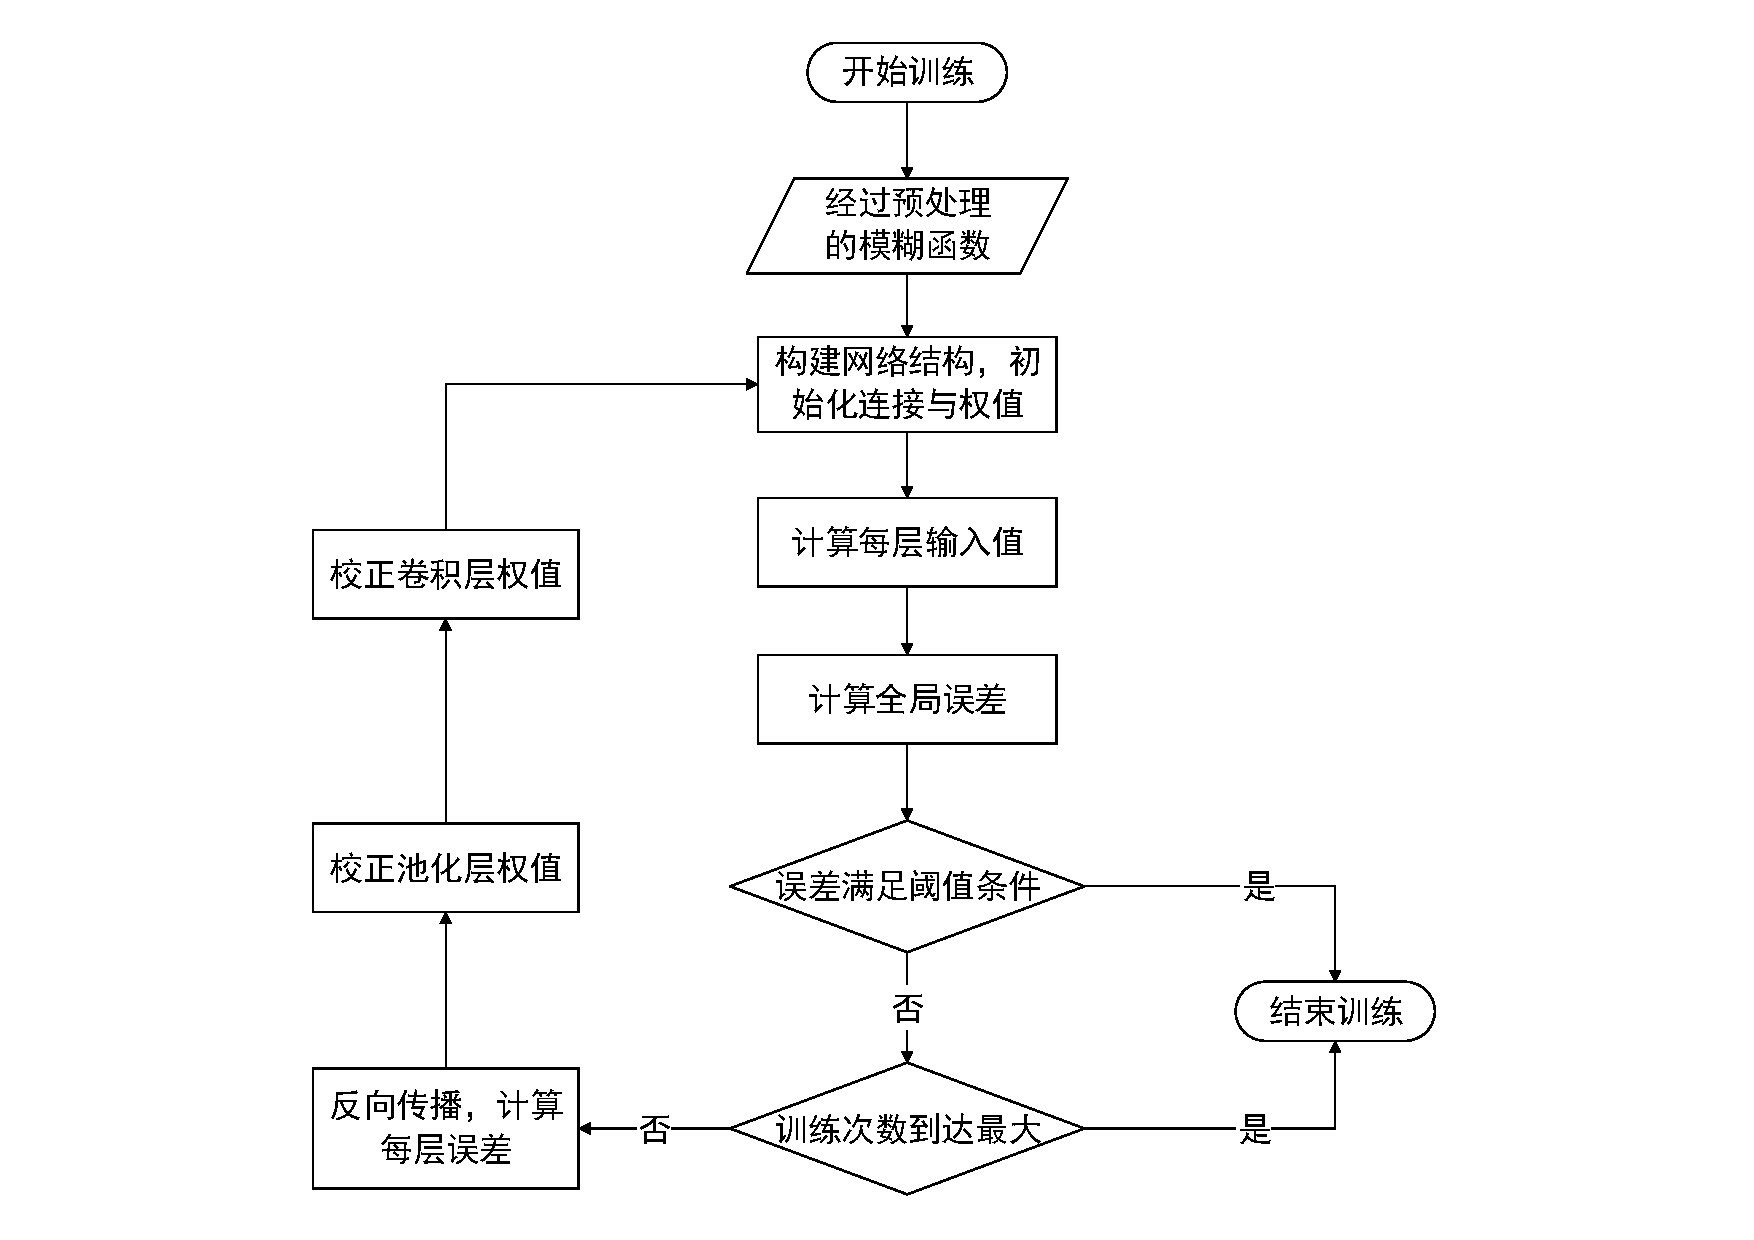
\includegraphics[width=\textwidth]{figures/cnn_flow.pdf}
	\caption{深度卷积神经网络算法训练流程图}
\end{figure}
将上述问题一般化也就是,最小化任意的具有 $m $个变量的多元实值函数 $C(v) $, $v=v_1,v_2,\dots,v_m $。对于这种具有大量变量的函数的解析解是极其复杂的,其比较合理的思路为利用数值计算的方法求取其极值点。每次对于$C $ 中的自变量 添加一个微小的变化$\Delta v $ ,根据此变化反映出来的$C $ 的变换 $\Delta C $更新下次的微小变化,从而使得$C $ 可以持续减小。对$C $ 中自变量的变化$\Delta v=(\Delta v_1,\dots,\Delta v_m)^T $ , $\Delta C $将会变为
\begin{equation}
    \Delta C \approx \bigtriangledown C \cdot \Delta v   
\end{equation}
,这里的梯度$\bigtriangledown C $ 定义如下:
\begin{equation}
\bigtriangledown C \equiv (\frac{\partial C}{\partial v_1},\dots,\frac{\partial C}{\partial v_m})^T 
\end{equation}
其把$v$的变化关联为$C$的变化,假设我们选取
$\Delta v=-\eta \bigtriangledown C $
这里的$\eta $是学习率,一般取一个很小的正数,这时候有
\begin{equation}
\Delta C \approx -\eta\bigtriangledown C\cdot\bigtriangledown C=-\eta||\bigtriangledown C||^2 \leq 0  
\end{equation}
也即如果利用更新规则
$v \rightarrow v'=v-\eta \bigtriangledown C$,
$C $会持续减小,此更新规则即为梯度下降算法,这就是最基本的学习算法。可以根据选择不同的代价函数 $C $或者通过计算来完成学习速率的选择等各种技术对学习算法进行优化。

% \begin{figure}[H]
% 	\centering
% 	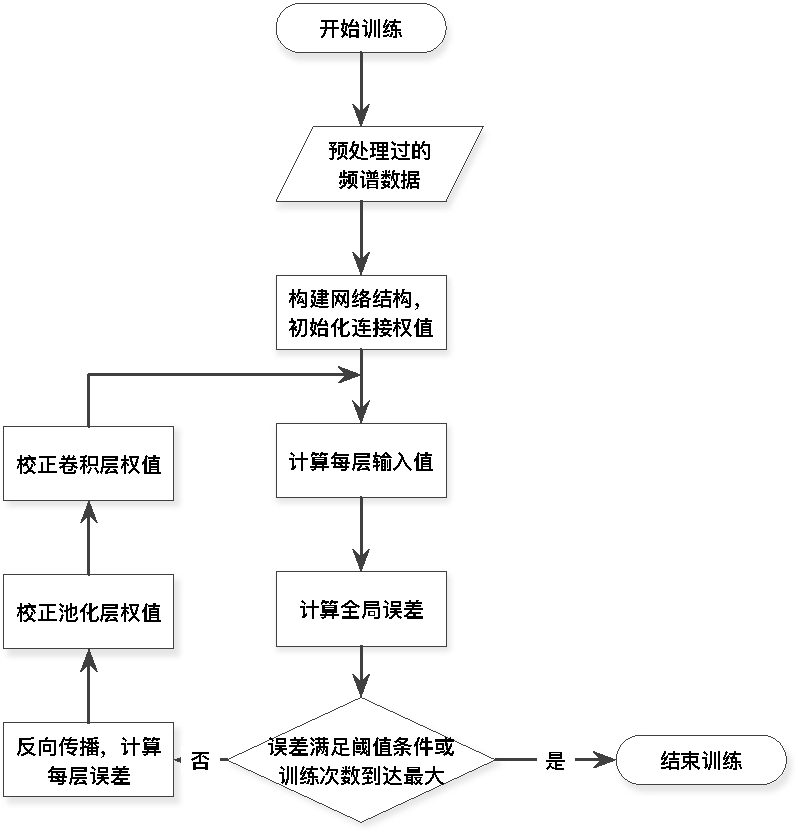
\includegraphics[width=\textwidth]{figures/train}
% 	\caption{深度卷积神经网络训练过程图}
% 	\label{fig:train}
% \end{figure}

\section{小结}
本章介绍了深度学习的相关基础。首先是其基本分类,然后针对于本文利用的深度卷积神经网络,介绍了传统的神经元的结构和卷积神经网络基于此的改进。在最后讨论了深度卷积神经网络在雷达信号处理中的应用。
% \begin{table}
%  \caption{测试表格}
%  \centering
%  \begin{tabular}{cccccc}
%    \toprule
%    & $h$ & $L^2$ error & Order & $L^{(\alpha,\beta)}$ error & Order \\
%    \midrule
%    \multirow{5}{4em}{$\alpha=0.85$\\ $\beta = 0.85$}
%    & 1/4   & 3.8571e-04 &      - & 3.0781e-03 &      -\\
%    & 1/8   & 1.3035e-04 & 1.5651 & 1.2640e-03 & 1.2840\\
%    & 1/16  & 3.8665e-05 & 1.7533 & 5.2782e-04 & 1.2599\\
%    & 1/48  & 4.9386e-06 & 1.8731 & 1.5519e-04 & 1.1142\\
%    \bottomrule
%  \end{tabular}
% \end{table}



% 参考文献设置
\clearpage
\phantomsection
\addcontentsline{toc}{chapter}{\fHei 参考文献}
\sWuhao
% npu专用
\bibliographystyle{nputhesis}
% 参考文献位置
\bibliography{references/reference}

% 附录
\backmatter
感谢XXX...
\phantomsection
\chapter*{毕业设计小结}
\addcontentsline{toc}{chapter}{\fHei 毕业设计小结}

毕业论文是大学四年的最后一份大作业...

\clearpage
\endinput

\clearpage
\end{document}
